\documentclass[11pt]{standalone}

\usepackage{amsmath}
\usepackage{ifthen}
\usepackage{tikz} 
\usetikzlibrary{shapes.misc}
\usetikzlibrary{arrows,arrows.meta}
\usetikzlibrary{calc,intersections, patterns, math}

\definecolor{pfeil}{RGB}{168,167,167}
\definecolor{petrol}{RGB}{0, 118, 136}
\definecolor{darkgoldenrod}{RGB}{184, 134, 11}
\colorlet{petrol-lighter}{petrol!40}
\colorlet{darkgoldenrod-lighter}{darkgoldenrod!40}

\renewcommand{\d}{\text{\,d}}

\begin{document}

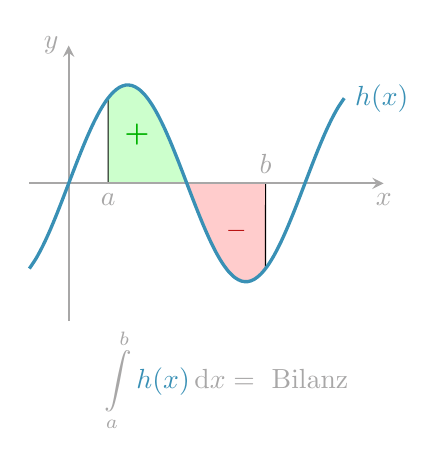
\begin{tikzpicture}[pfeil]

    % \draw[thick, fill=petrol!20, draw=petrol-lighter, rounded corners=2ex, opacity=0.5] (0,0) rectangle ++ (1.5,3.5);
    % \draw[thick, fill=darkgoldenrod!20, draw=darkgoldenrod-lighter, rounded corners=2ex, opacity=0.5] (5,0) rectangle ++ (1.5,3.5);

    % \draw[thick, -stealth] (-4.5,0) -- (4.5,0) node[below]{$\scriptstyle x$};
	% \draw[thick, -stealth] (0,-2.5) -- (0,2.5) node[left]{$\scriptstyle y$};
	
	\path[domain=0.5:1.5, thin, draw=black, fill=green!20] (0.5,0) -- plot(\x,{1.25*sin(2/3*pi*\x r)}) -- (1.5,0) --cycle;
		\path[domain=1.5:2.5, thin, draw=black, fill=red!20] plot(\x,{1.25*sin(2/3*pi*\x r)}) -- (2.5,0) --cycle;
		\draw[thick,-stealth] (-0.5,0) -- (4,0) node[below]{$x$};
		\draw[thick,-stealth] (0,-1.75) -- (0,1.75) node[left]{$y$};
		\node[below] at (0.5,0) {$a$};
		\node[above] at (2.5,0) {$b$};
		\node[green!70!black] at (0.866,0.625) {\textbf{+}}; 
		\node[red!70!black] at (2.1333,-0.625) {\textbf{--}}; 
		\draw[domain=-0.5:3.5, very thick, cyan!70!black, samples=50, smooth] plot(\x,{1.25*sin(2/3*pi*\x r)}) node[right] {$h(x)$};
		\node at (2,-2.5) {$\displaystyle\int\limits_a^b {\color{cyan!70!black}h(x)} \d x = \text{ Bilanz}$};

\end{tikzpicture}

\end{document}
